\vspace*{-.25em}

\section{Preliminary Study}

% Introduce the schemas and the give the basic layout of the experiments and how they are visualized

To demonstrate the effectiveness and domain extensibility of \mrstudyr, we studied the mutants of the nine schemas in
Table~\ref{tbl:study-schemas} with the presented tool. Similar to the studies of Wong and
Mathur~\cite{mathur1994empirical}, \mr~performed mutant sampling with $x$ value increments larger than $1\%$.
Specifically, for this experiment, \mr~analysed $x$ at $1\%$ and $10\%$, then increased by $10\%$ intervals to a maximum
value of $90\%$. By setting the granularity of the experiment to $10\%$ intervals, \mr~reduces the cost of performing
retrospective analysis, while confirming trends from prior work, as shown in Figure~\ref{fig:graph}. For each of the
sampling techniques currently supported by \mr, the mutant reducer is invoked at each $x$ percentage for each of the
schemas under test for a total of 30 trials.

% Fully explain the structure of the boxplot (but, there are additional details in a subcaption of the figure)

Figure~\ref{fig:graph} is a box-and-whisker plot with the schemas on the horizontal-axis and the mutation scores of the reduced
sets after random sampling at the $x$ values of 1\%, 10\%, 20\%, and 40\% on the vertical-axis.  These values were chosen as the
$x$ values because they serve to confirm a previously observed trend of decreasing errors between the original and reduced sets'
mutation score as $x$ increases. Moving from top-left to bottom-right, the boxes in Figure~\ref{fig:graph} show this decrease in
error.

% by becoming more flat as $x$ increases.

% Go through all of the results in the graph

This trend occurs because the mutation scores of reduced sets with smaller percentages are often very volatile and can
thus vary largely based on one or few mutants; in contrast, the mutation scores of sets with greater percentages are
substantially more stable. In the top-left of Figure~\ref{fig:graph}, $x$ is evaluated at 1\%. In this quadrant of
Figure~\ref{fig:graph}, the calculated RMSE, 12.090, is very high with respect to the same metric at greater
percentages, while the correlation coefficient, 0.385, is considered to be ``low'' according to Guildford scale. In
the top-right quadrant, where $x$ is 10\%, stability is already evident in the reduced sets' mutation scores. At this
percentage, an RMSE of 4.082, is much lower than at 1\% and correlation is ``high'' with a coefficient value of 0.654.
This same trend of decreasing RMSE values and increasing correlation coefficients remains true for $x$ values of 20\%
and 40\%. At 20\% and 40\%, RMSE is 2.485 and 1.568 and the correlation coefficients are ``very high'' for both,
with values of 0.763 and 0.852, respectively.

% But, if you want to confirm our results, the tool is available for you to run yourself!

These results demonstrate that it is possible to easily use \mr~to confirm the prior results of Wong and Mathur in the
new application domain of database schemas. More studies can now be run as \mr~is available from GitHub~\cite{tool}.

\begin{figure}[!t]

  \centering
  \hspace*{-1em}

  \begin{minipage}{4in}
    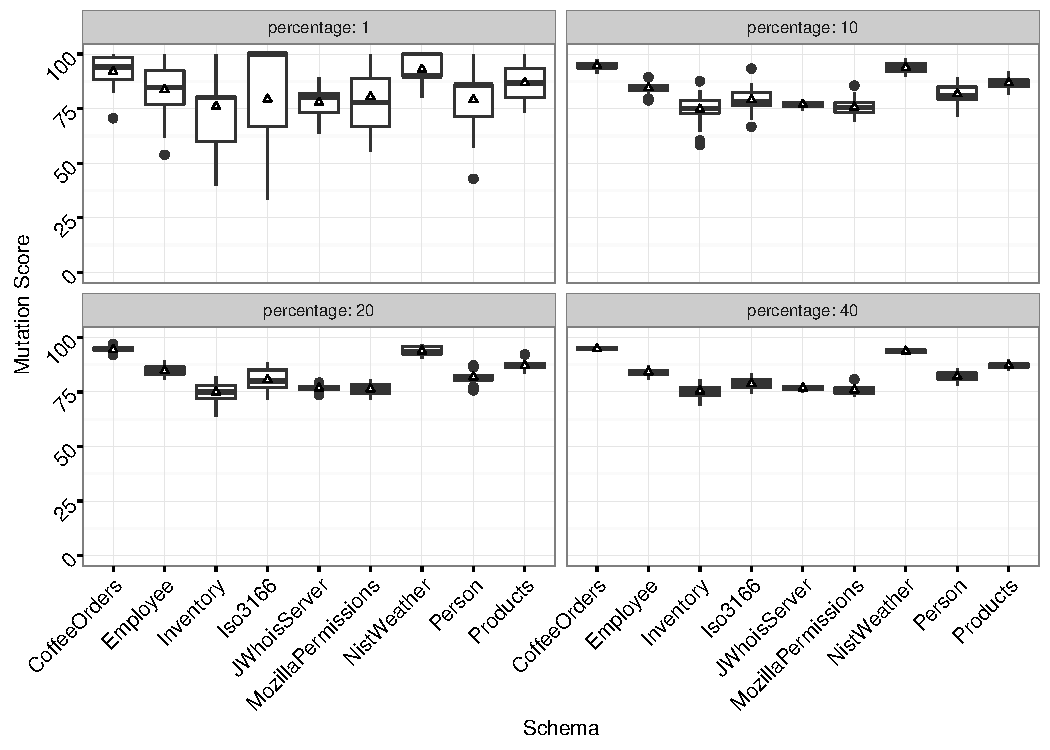
\includegraphics[scale = 0.5]{graphs/schema_vs_ms.pdf}
  \end{minipage}

  \caption{\label{fig:graph}Graph displaying mutation scores for database schemas.}

  \vspace{-1.8em}

\end{figure}

